\section{Fast Multipole Methods (FMMs)}

\subsection{Motivation}

\begin{frame}{Motivation - the $N$ Body Problem}
    \begin{itemize}
        \item e.g. Electrostatics, Gravitation
        \item $\{ x_i \}_{i=1,..,N}$ Source Particles
        \item $\{ y_j \}_{j=1,..,M}$ Target Particles
    \end{itemize}

    \begin{flalign}
        &\Phi(y_j) = \sum_{i=1}^N K(x_i, y_j) q_i, \\
        &\text{where,  } K(x, y) = \frac{1}{\|x-y\|}
    \end{flalign}

    \begin{itemize}
        \item FMM reduces complexity from $O(N^2)$ to $O(N)$
    \end{itemize}
    \vspace{50pt}
\end{frame}

\begin{frame}{Motivation - Intuition}
    \begin{figure}
        \centering
        {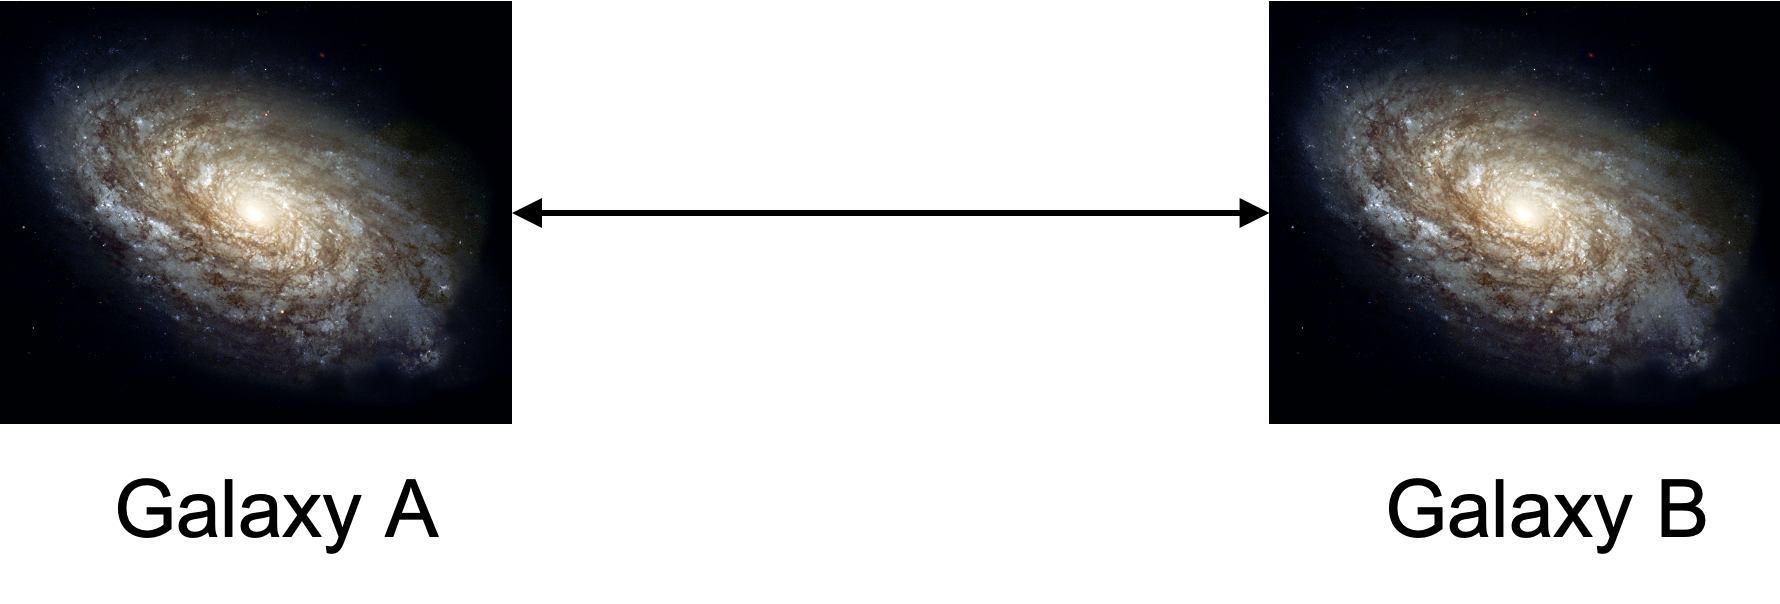
\includegraphics[width=0.8\textwidth]{assets/galaxy.png}}
    \end{figure}
\end{frame}

\begin{frame}{Motivation - Intuition}
    \begin{figure}
        \centering
        {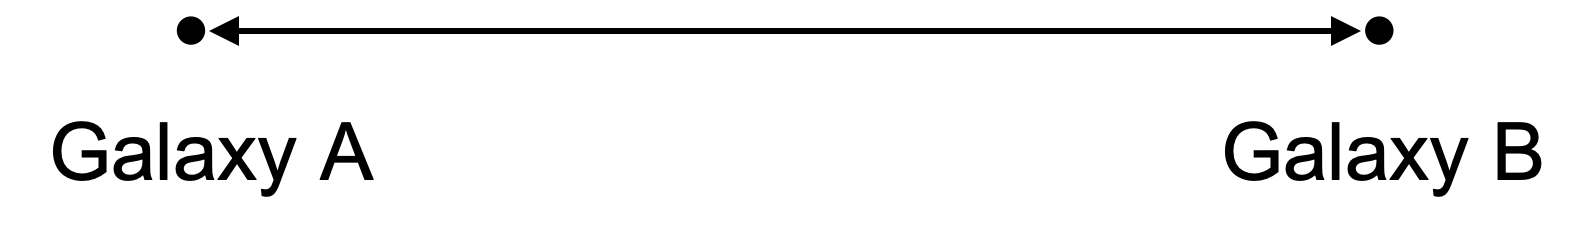
\includegraphics[width=0.8\textwidth]{assets/dot.png}}
    \end{figure}
\end{frame}

\begin{frame}{Motivation - Three Step Procedure}
    \begin{figure}
        \centering
        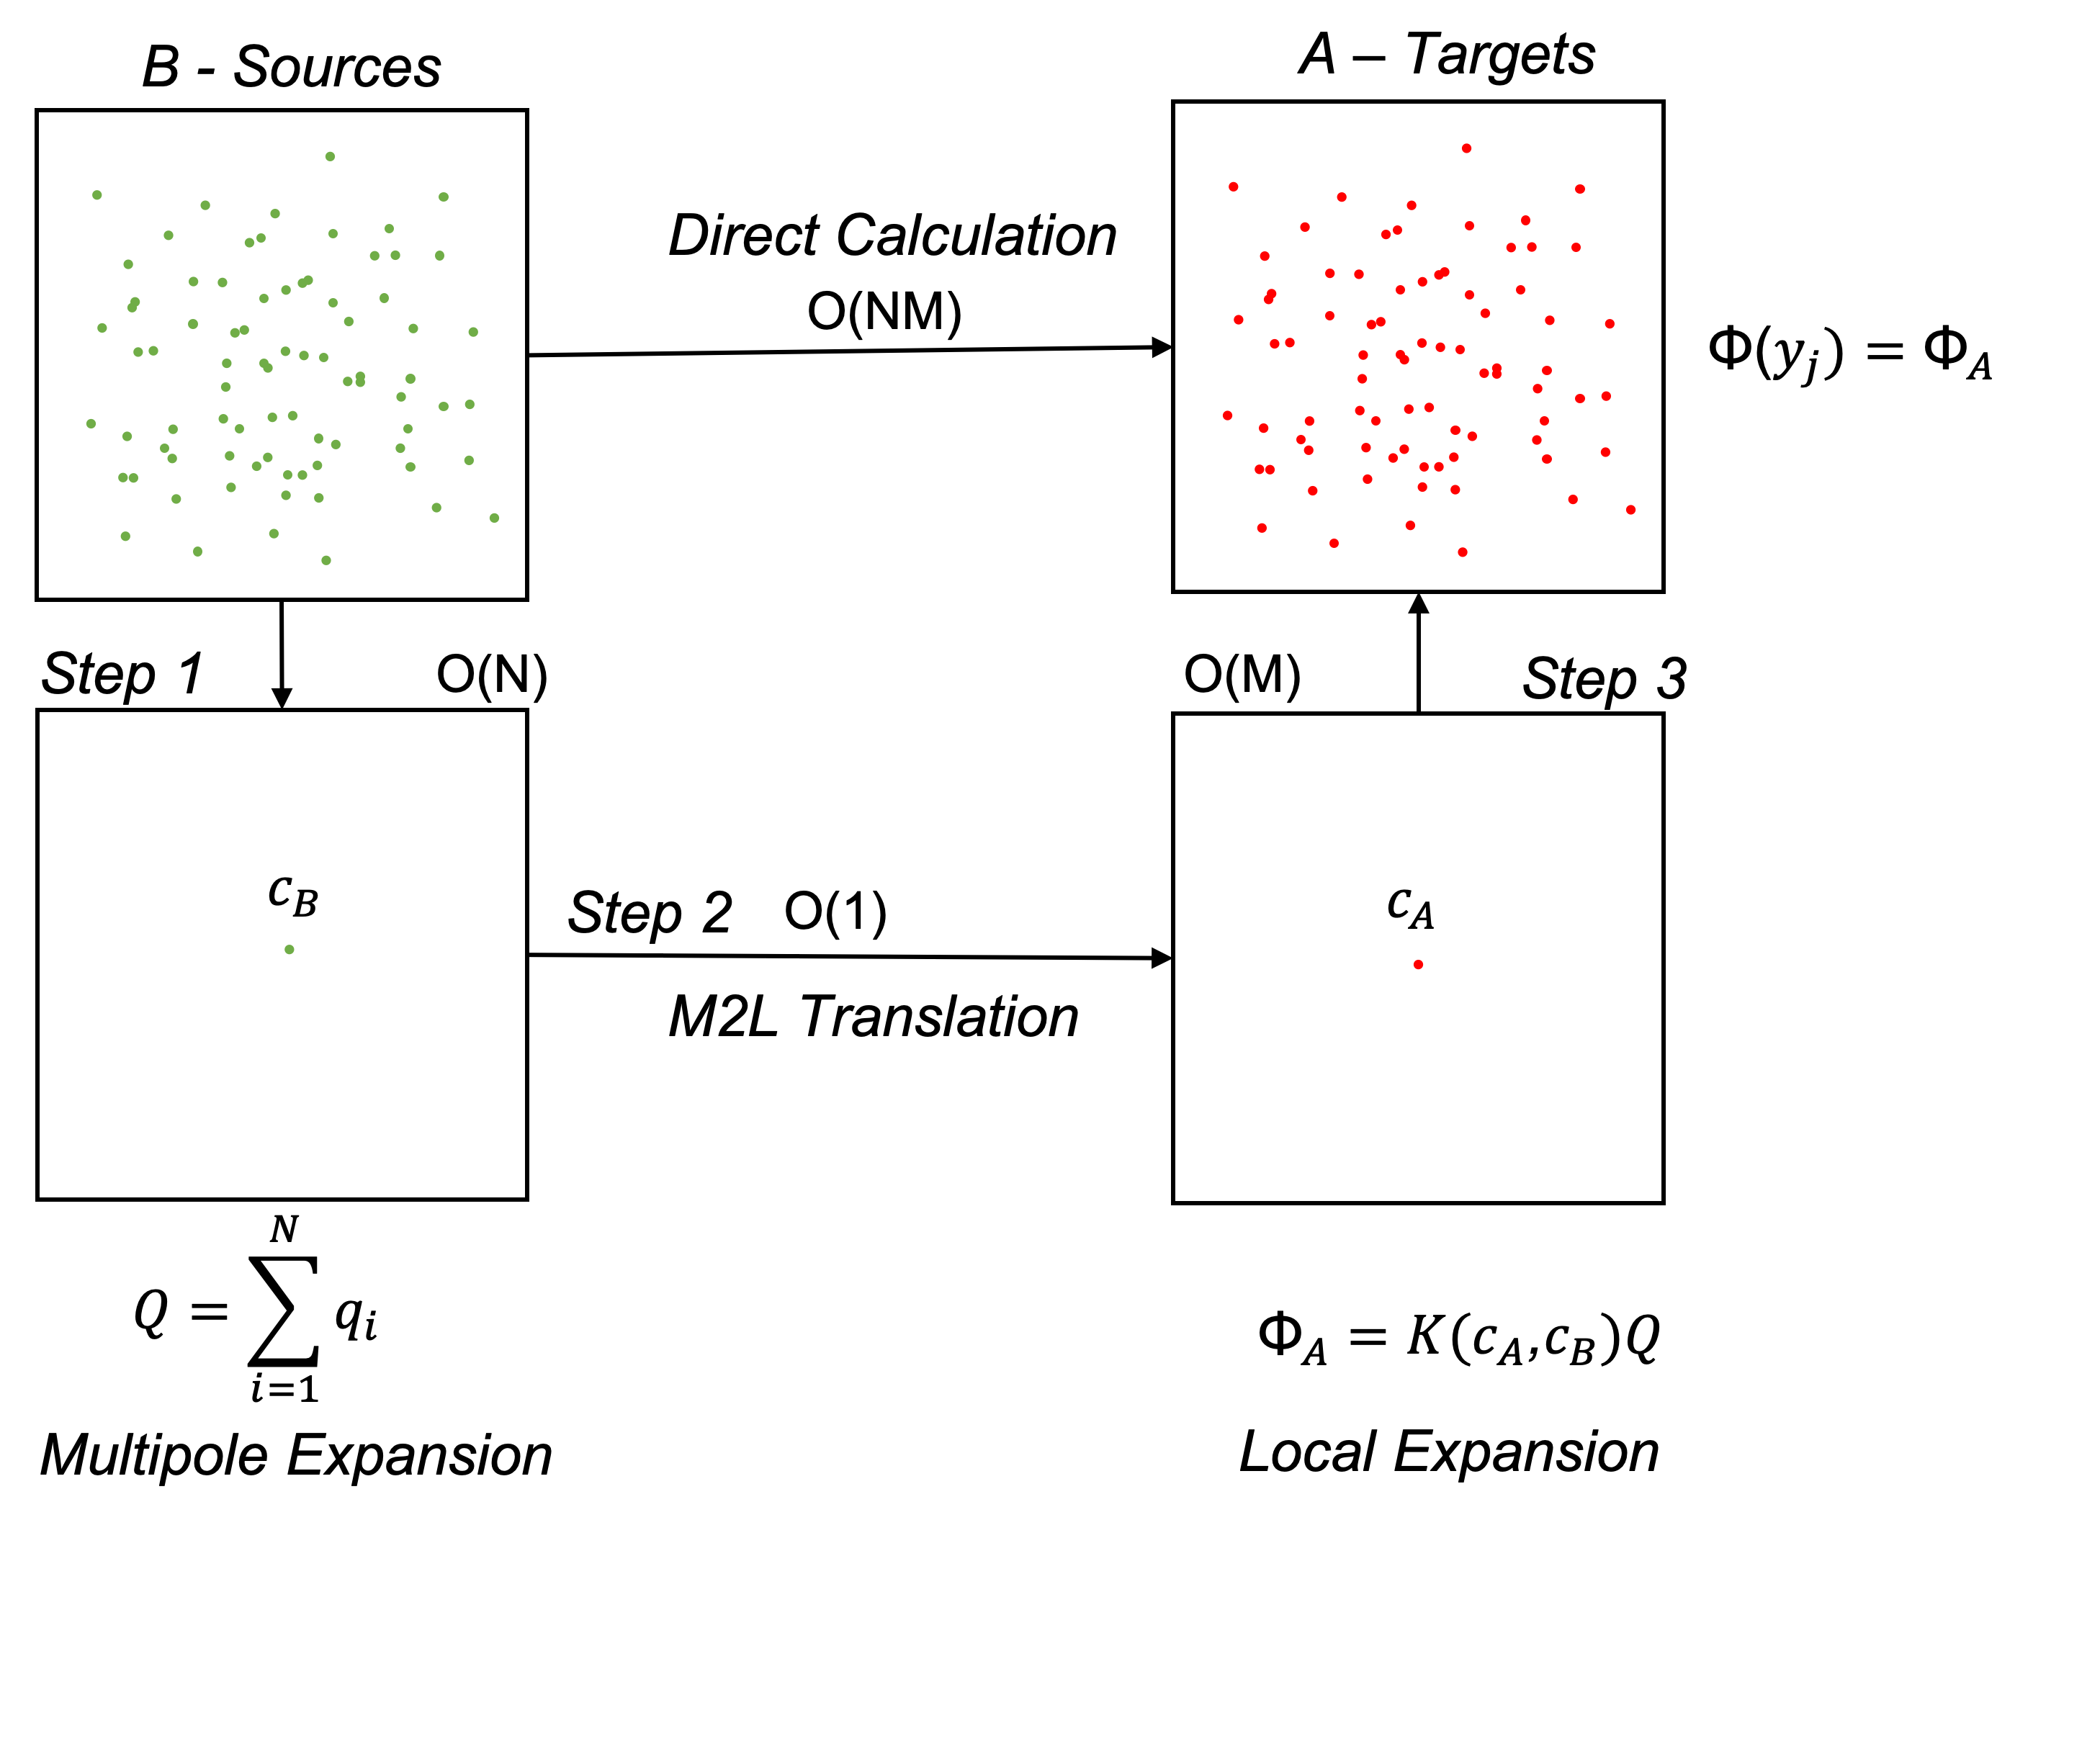
\includegraphics[width=0.8\textwidth]{assets/three_step.png}
    \end{figure}
    \vspace{50pt}
\end{frame}

\subsection{Analytic FMM}
\begin{frame}{Analytic FMM - Concept}
    \textbf{Idea}: Use compressed representations of far field potentials to reduce complexity, in a recursive fashion
\end{frame}

\begin{frame}{Analytic FMM - Multipole Expansion}
    \begin{figure}
        {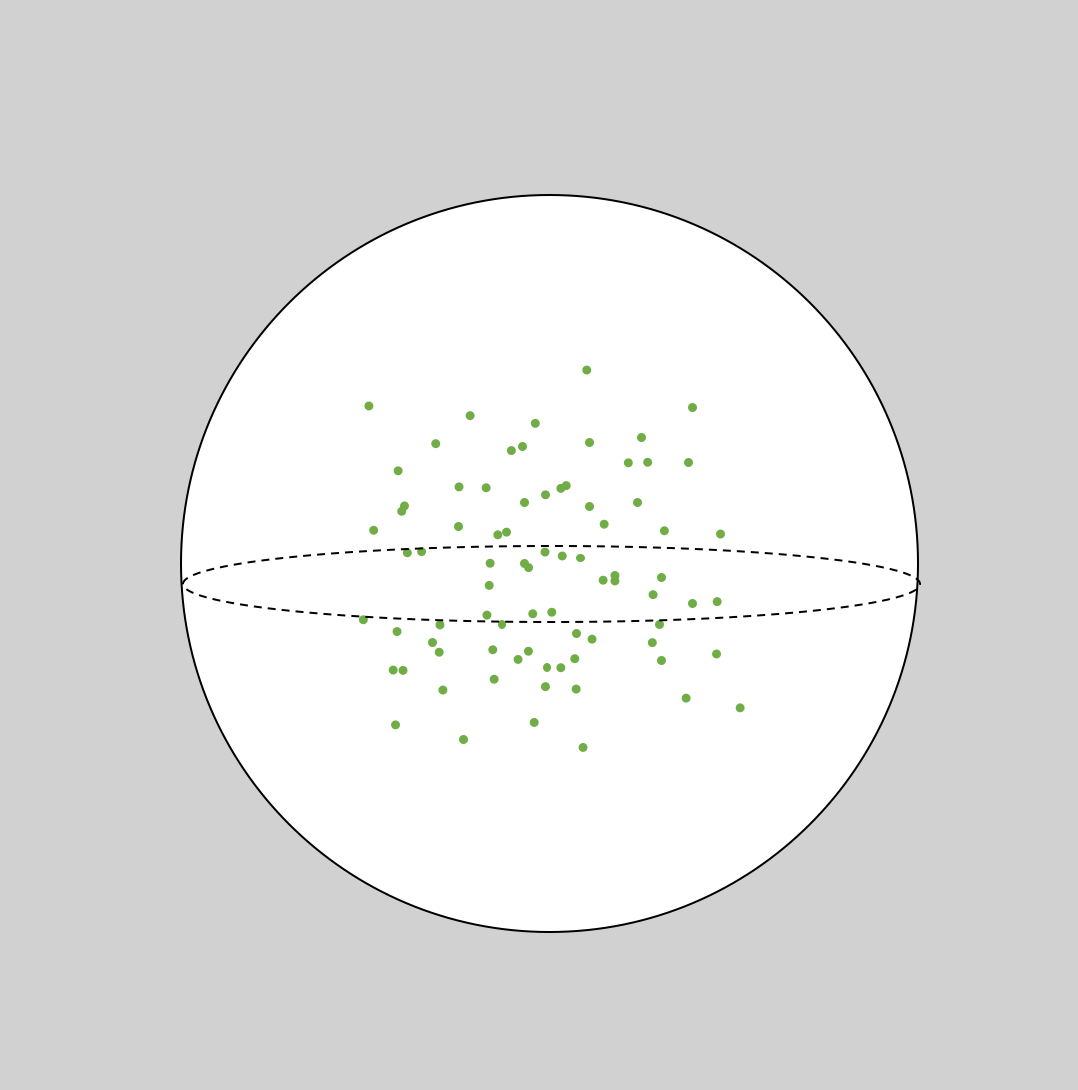
\includegraphics[width=0.5\textwidth]{assets/multipole.png}}
        \vspace{50pt}
    \end{figure}
\end{frame}


\begin{frame}{Analytic FMM - Local Expansion}
    \begin{figure}
        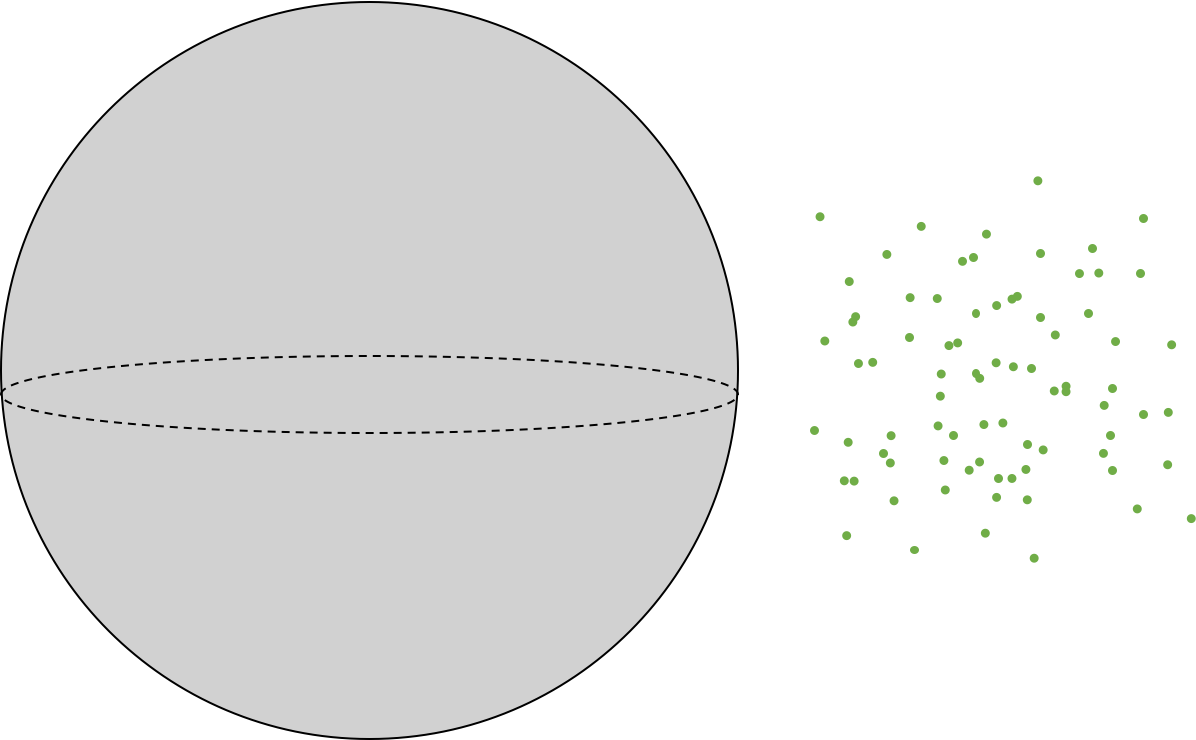
\includegraphics[width=0.7\textwidth]{assets/local.png}
    \end{figure}
\end{frame}

\begin{frame}
    \begin{itemize}
        \item For 3D Laplace kernel, can write multipole and local expansions using sph. harmonics, these can be truncated to required accuracy
        \item Exact operators exist for this kernel to shift between multipole and local expansion coefficients
        \item Exact bounds on error also exist, with respect to direct computation \cite{Greengard:1987:JCP}
    \end{itemize}
\end{frame}

\begin{frame}{Analytic FMM - Motivating Problem}
    \begin{itemize}
        \item Consider 2D Problem
        \item Domain, $\Omega = [0,1] \times [0, 1]$
        \item Partition into recursively defined Quadtree
        \item Each level, $l$, partitioned into $4^l$ boxes
        \item Source and Target particles taken to be the same
    \end{itemize}
\end{frame}

\begin{frame}{Analytic FMM - Shifting Multipole Expansion}
    \begin{figure}
        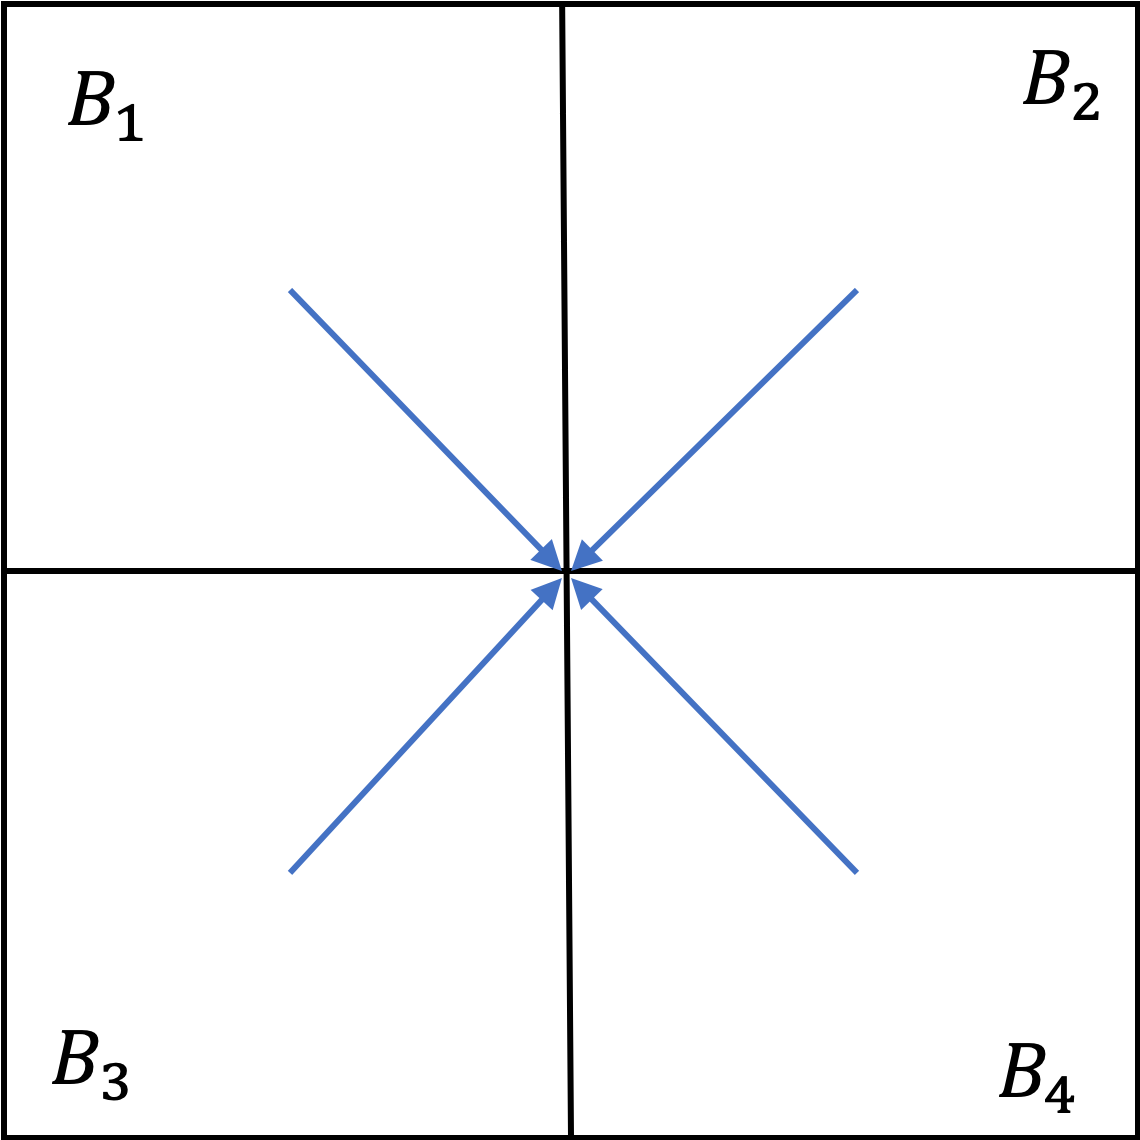
\includegraphics[width=0.5\textwidth]{assets/multipole_shift.png}
        \vspace{50pt}
    \end{figure}
\end{frame}

\begin{frame}{Analytic FMM - Shifting Local Expansion}
    \begin{figure}
        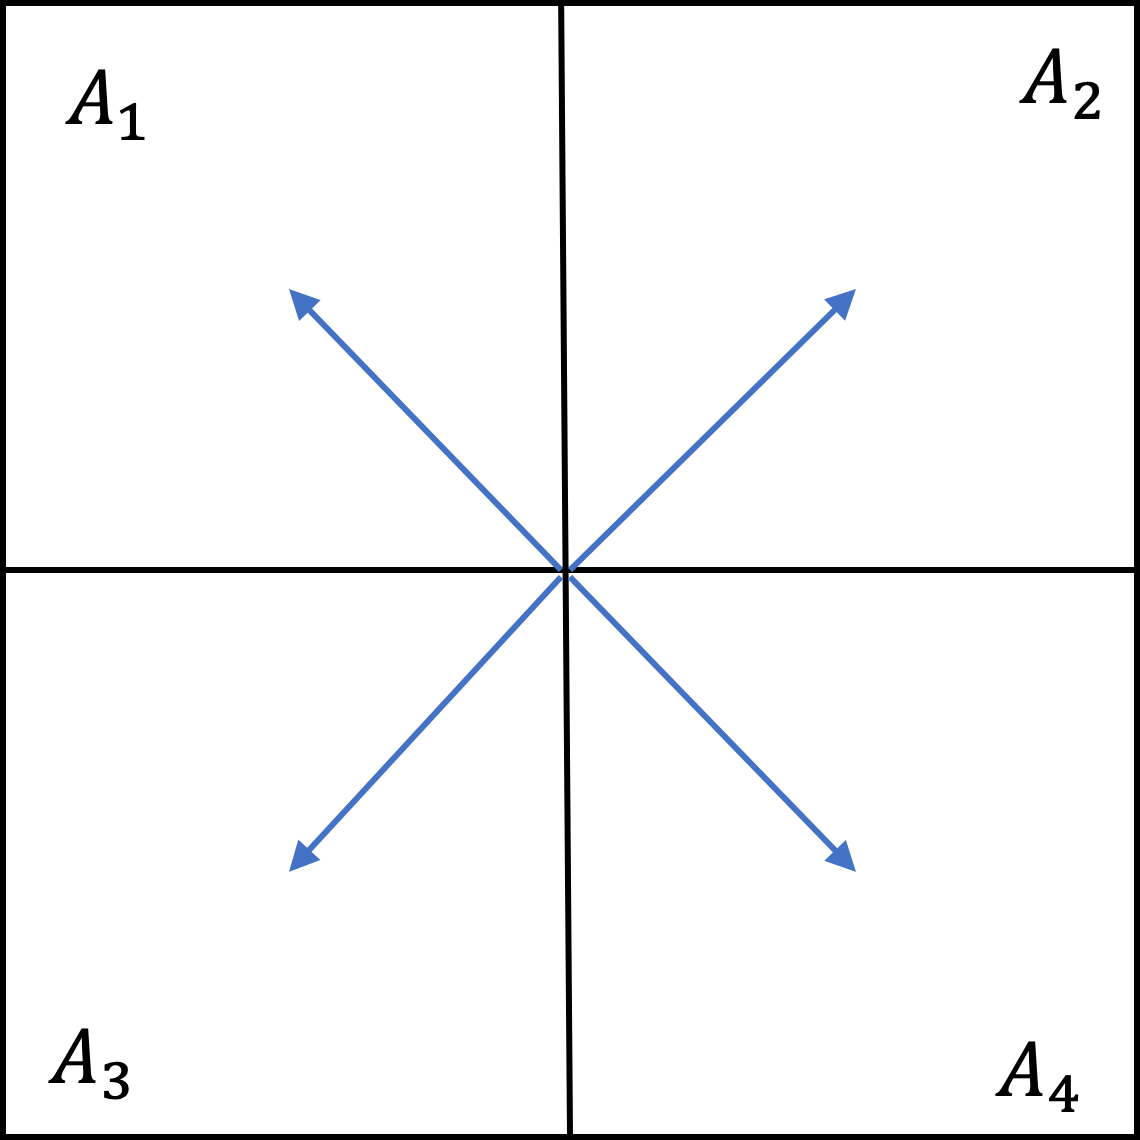
\includegraphics[width=0.5\textwidth]{assets/local_shift.png}
        \vspace{50pt}
    \end{figure}
\end{frame}

\begin{frame}
    \begin{figure}
        \centering
        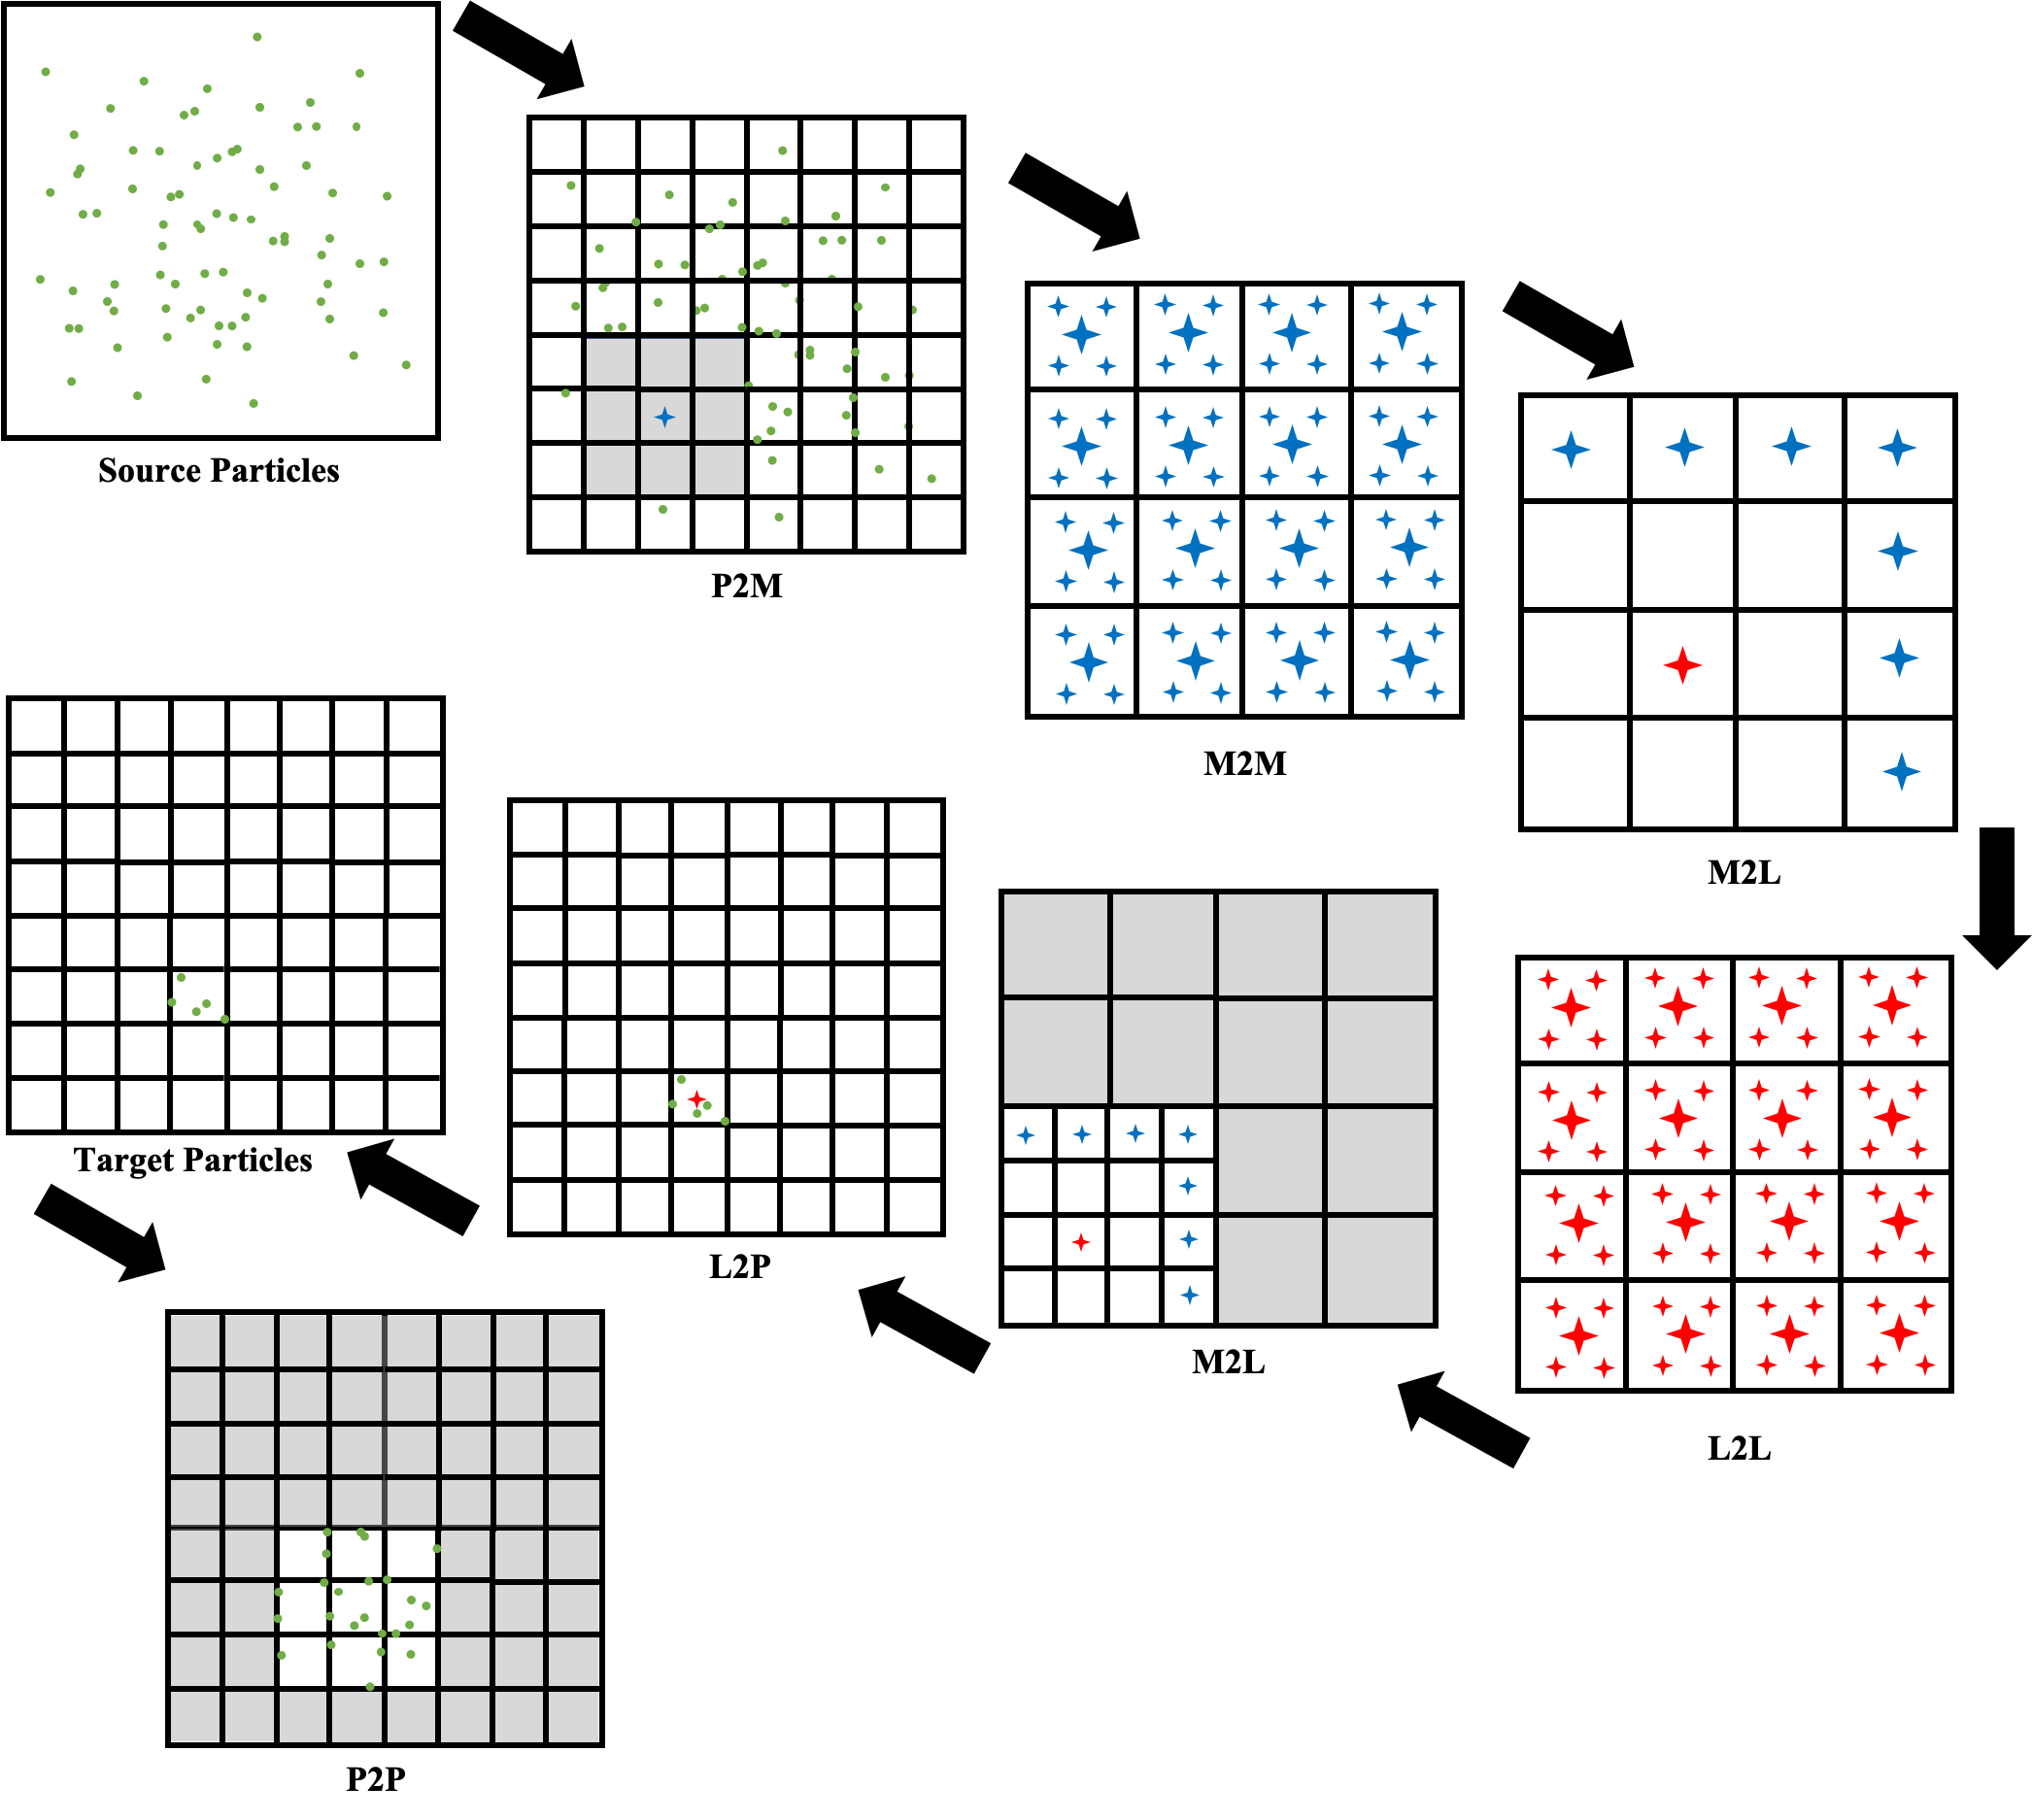
\includegraphics[width=0.7\textwidth]{assets/main_loop.png}
    \end{figure}
    \vspace{50pt}
\end{frame}

\begin{frame}{Analytic FMM - Implementation Issues}
    \begin{itemize}
        \item Representing problem with efficient data structures: Quad/Octrees
        \item Computing and storing new expansions for each kernel, may require new software implementations
    \end{itemize}
\end{frame}


\subsection{Kernel Independent FMM}
\begin{frame}{Kernel Independent FMM}
    \begin{itemize}
        \item KIFMM only requires kernel evaluations
        \item Works by matching potential generated by particles with that generated by an equivalent density in the far field
    \end{itemize}
\end{frame}

\begin{frame}{Kernel Independent FMM - Least Squares Problem}
    \begin{figure}
        \centering
        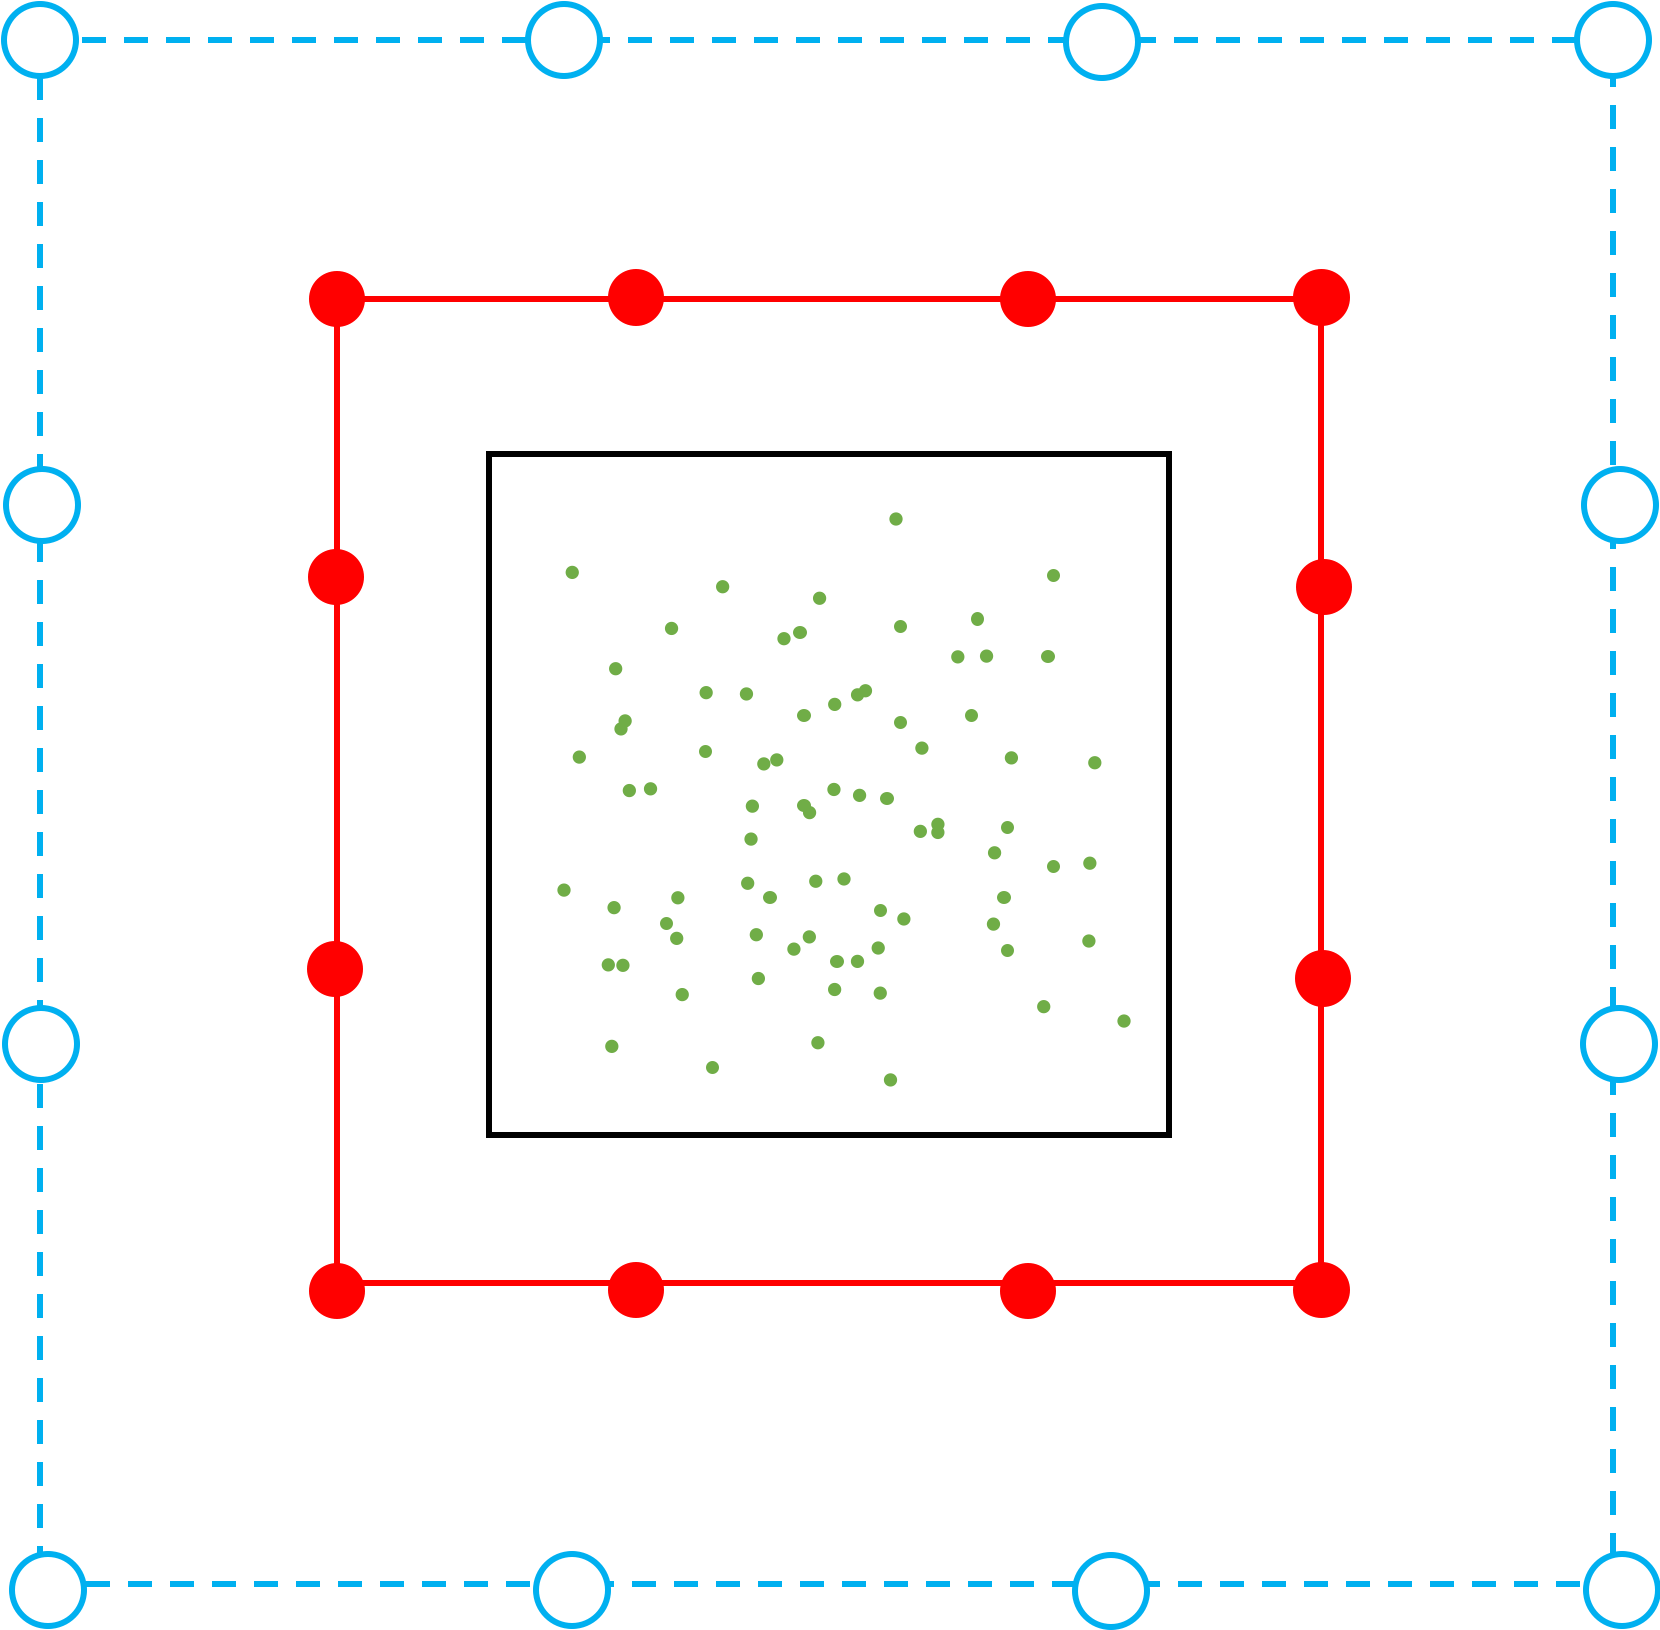
\includegraphics[width=0.5\textwidth]{assets/least_sq_multipole.png}
    \end{figure}

    Adapted from \cite{Ying:2004:JCP}

    \vspace{55pt}
\end{frame}

\begin{frame}{Kernel Independent FMM - Least Squares Problem}
    \begin{figure}
        \centering
        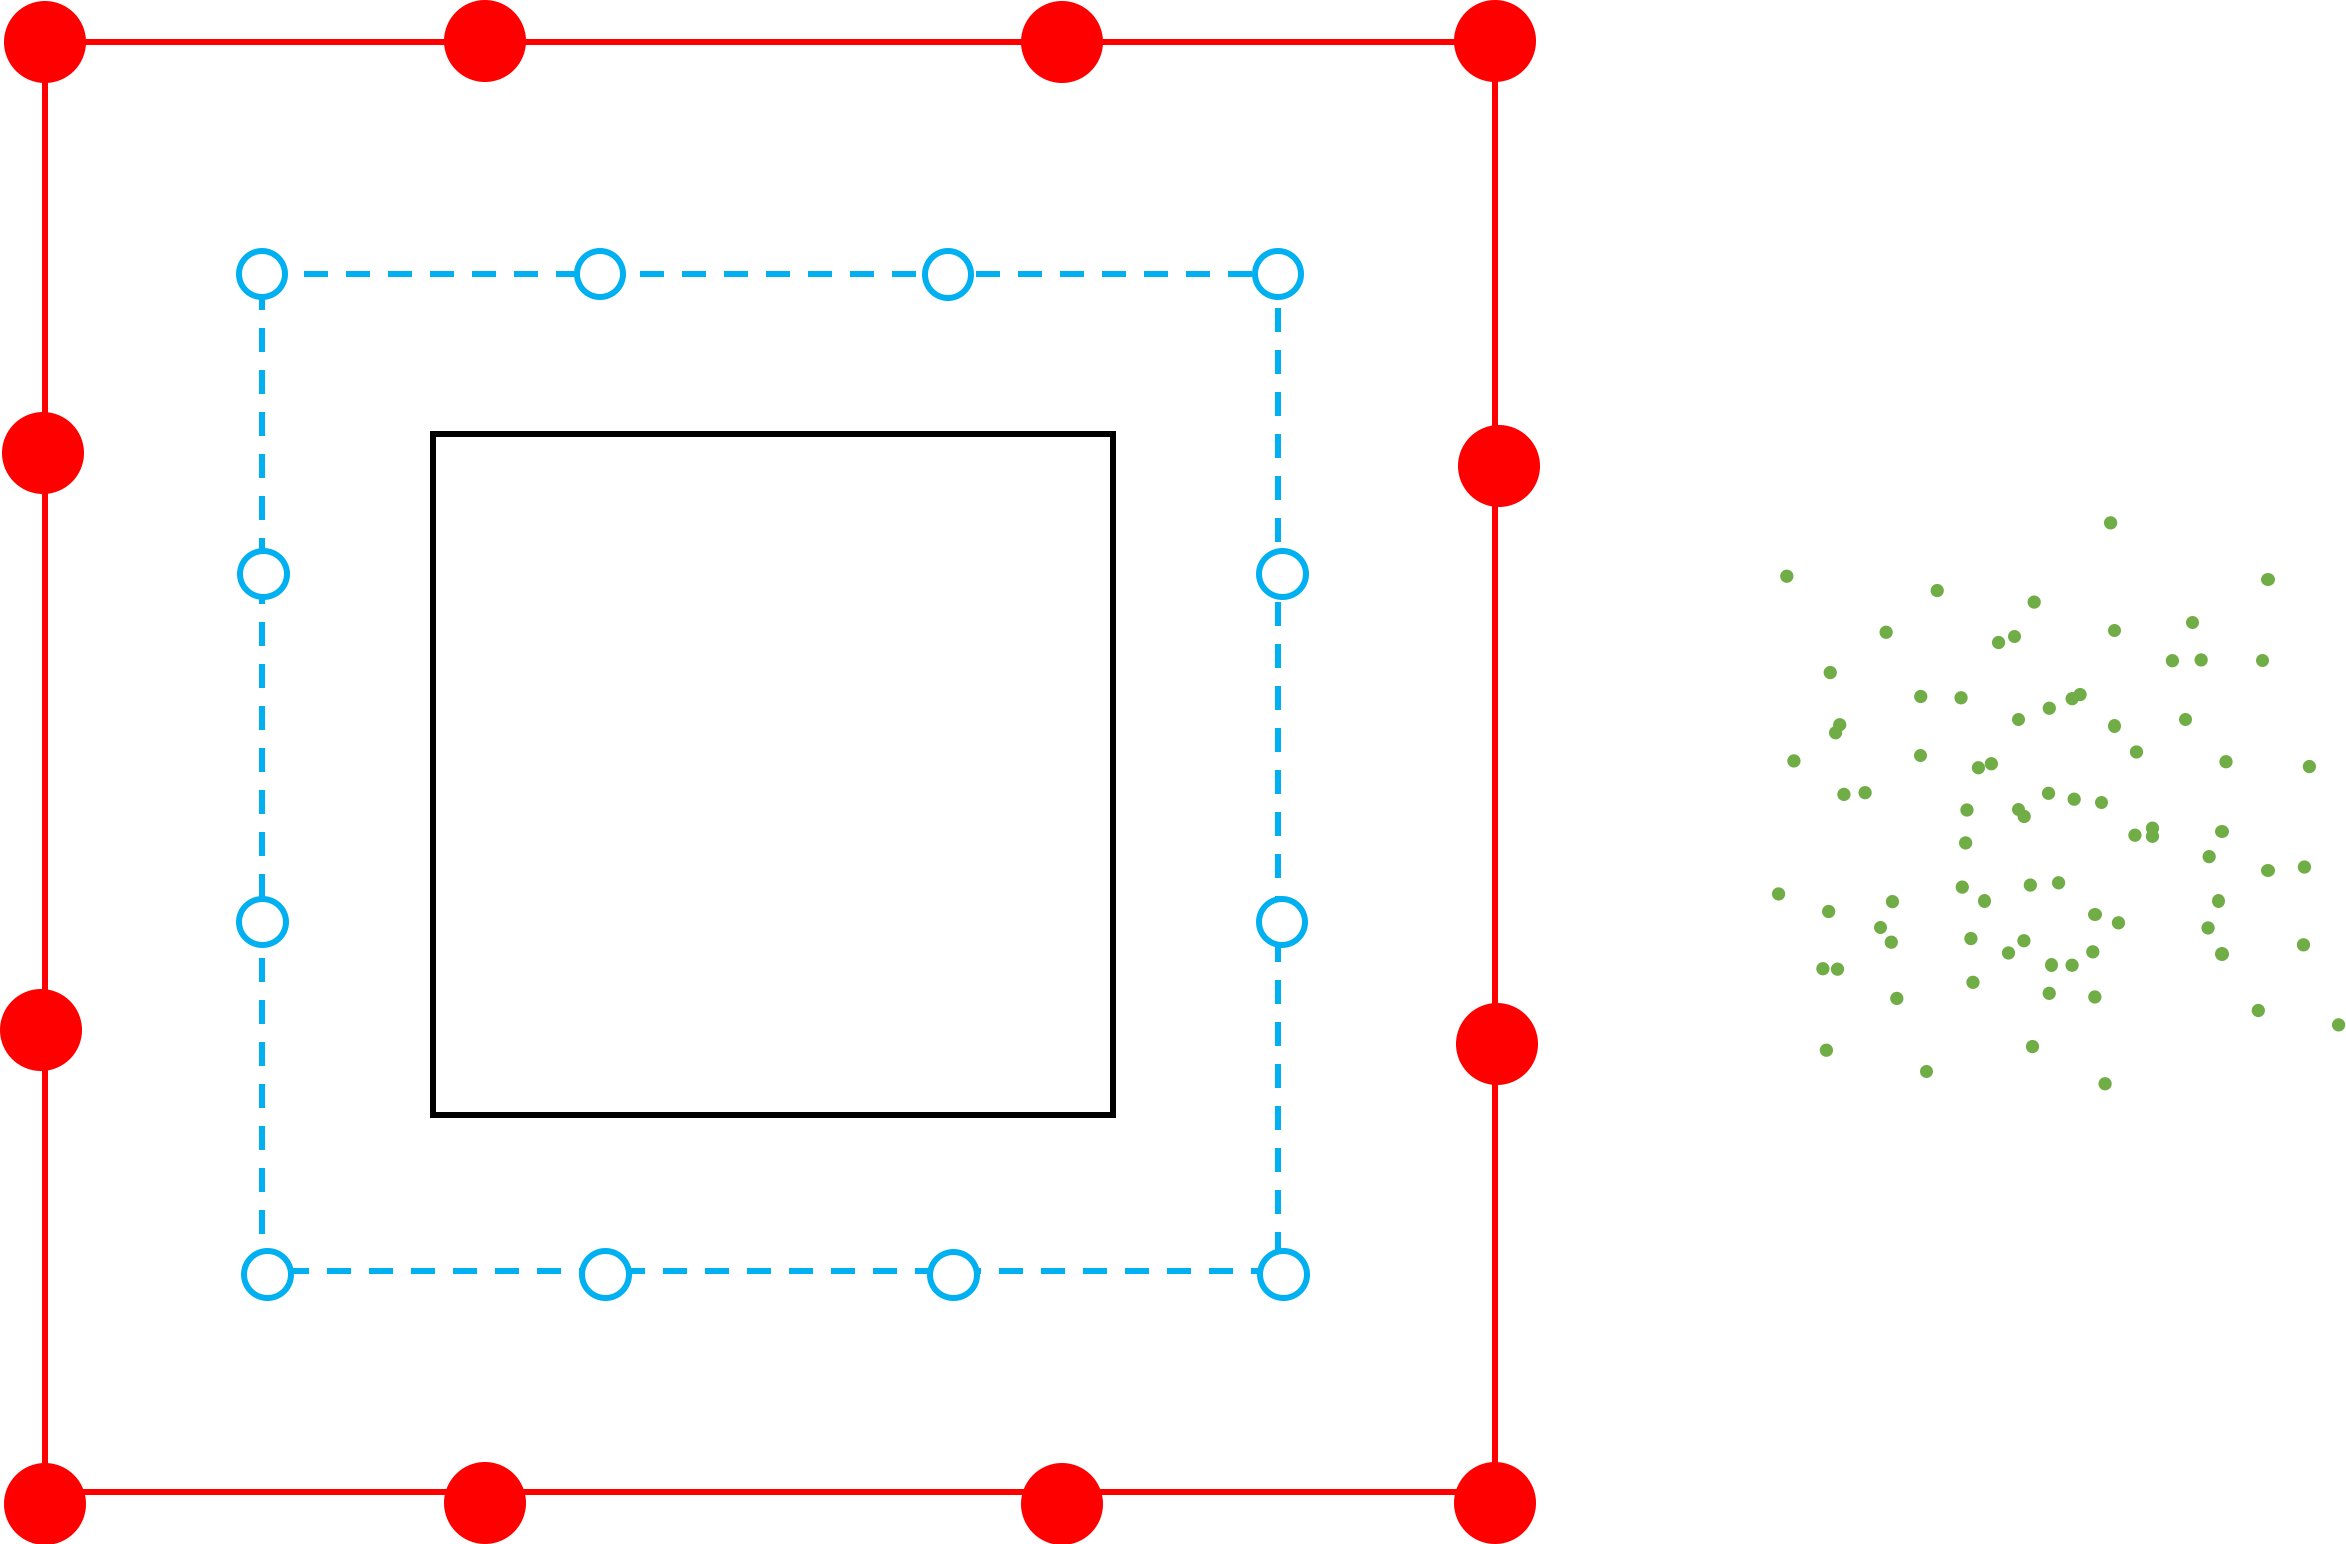
\includegraphics[width=0.7\textwidth]{assets/least_sq_local.png}
    \end{figure}

    Adapted from \cite{Ying:2004:JCP}
    \vspace{50pt}
\end{frame}

\begin{frame}{Kernel Independent FMM - Least Squares Problem}
    \begin{itemize}
        \item Check Surface $x^{B, u}$
        \item Equivalent Surface $y^{B, u}$
        \item Equivalent Density $\phi^{B, u}$
        \item Check Potential $q^{B, u}$
        \item Indices of source points $I_s^B$
        \item Source densities $\phi_i$
    \end{itemize}


    \begin{equation}
        \int_{\mathbf{y}^{B,u}} K(\mathbf{x}, \mathbf{y})\phi^{B, u} d\mathbf{y} = \sum_{i \in I_s^B} K(\mathbf{x}, \mathbf{y})\phi_i = q^{B, u} \> \> \text{for any} \> \> \mathbf{x} \in \mathbf{x}^{B, u}
    \end{equation}

\end{frame}

\begin{frame}{Kernel Independent FMM - Least Squares Problem}

    \begin{flalign}
        &K_A\phi^A = K_B\phi^B \\
        &\phi^A = (\alpha I + K_A^*K_A)^{-1}K_B\phi^B
    \end{flalign}

\end{frame}


\begin{frame}{Kernel Independent FMM - Least Squares Problem, M2L}

    \begin{figure}
        \centering
        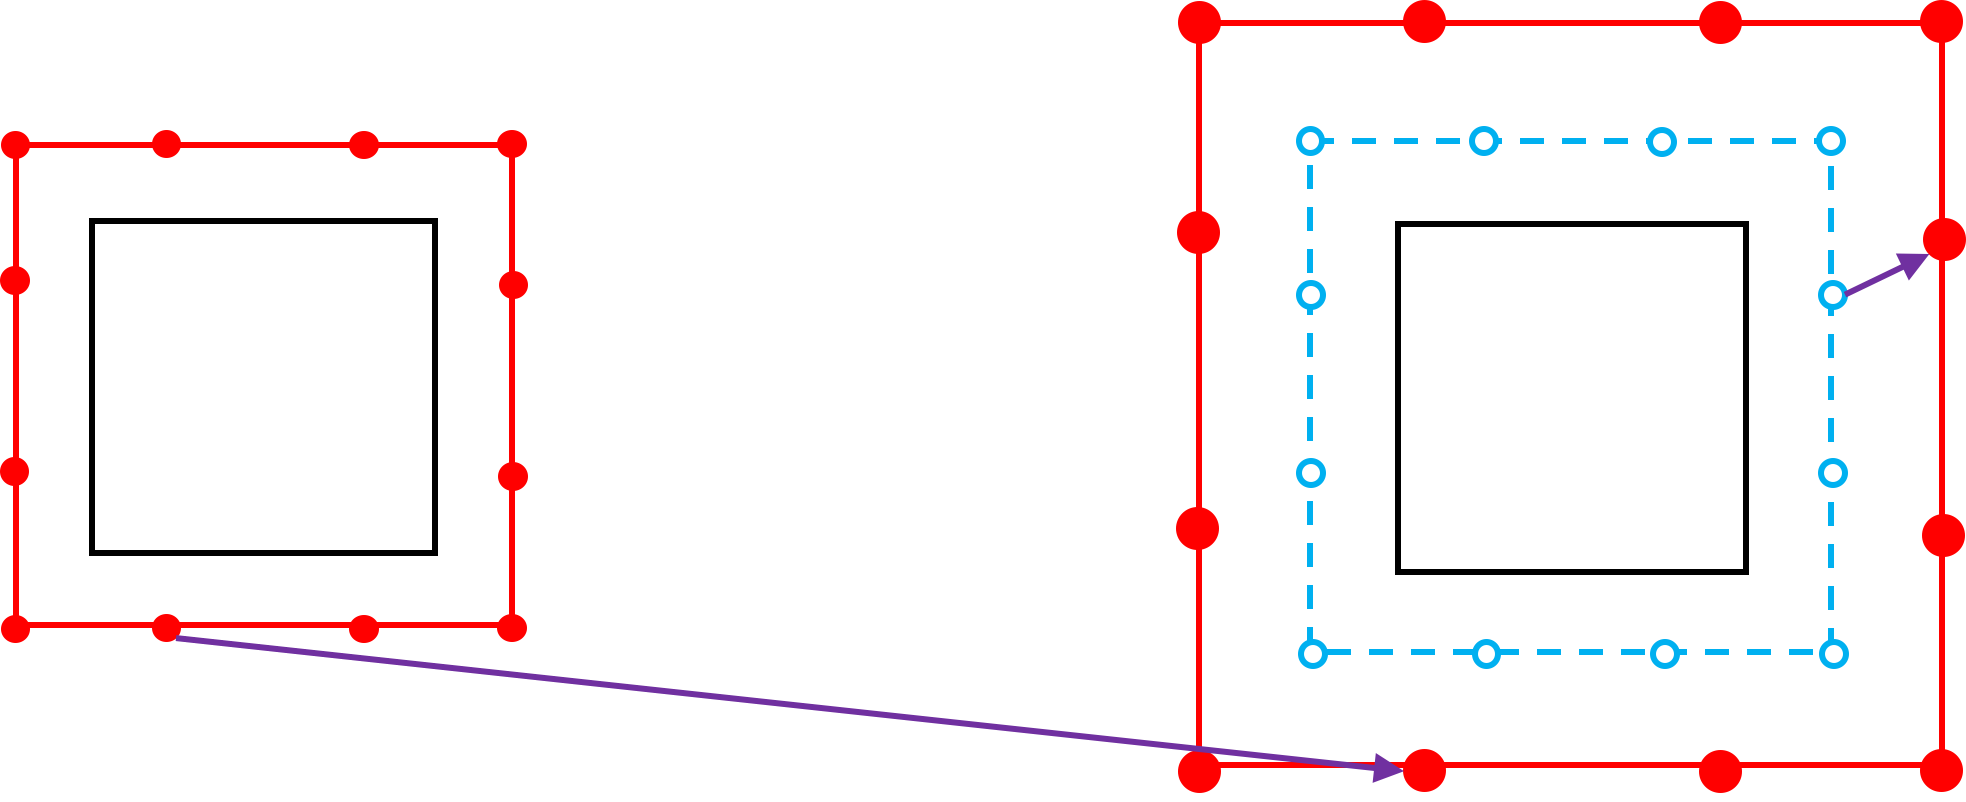
\includegraphics[width=0.7\textwidth]{assets/kifmm_m2l.png}
        \vspace{50pt}
    \end{figure}
\end{frame}

\begin{frame}{Kernel Independent FMM - Least Squares Problem, M2L}
    \begin{itemize}
        \item Check Surface $x^{B, u}$
        \item Downward Equivalent Surface $y^{B, d}$
        \item Upward Equivalent Surface $y^{A, u}$
        \item Downward Equivalent Density $\phi^{B, d}$
        \item Upward Equivalent Density $\phi^{A, u}$
    \end{itemize}


    \begin{equation}
        \int_{\mathbf{y}^{A,u}} K(\mathbf{x}, \mathbf{y})\phi^{A, u} d\mathbf{y} =   \int_{\mathbf{y}^{B,d}} K(\mathbf{x}, \mathbf{y})\phi^{B, d} d\mathbf{y}, \> \> \text{for any} \> \> \mathbf{x} \in \mathbf{x}^{B, d}
    \end{equation}
\end{frame}

\begin{frame}{Kernel Independent FMM - Implementation Issues}
    \begin{itemize}
        \item No need for new software implementation for large class of compatible Kernels
        \item Can built singly, extensible, and optimisable software implementation
    \end{itemize}
\end{frame}